\section{Dados de Validação}
Os dados de validação são os mesmos que os dados de treino, embora apenas durante os anos de 2019 a 2022, inclusive.\\
Usamos como benchmark as capacidades alocadas, "SecondaryReserveAllocationAUpward" e "SecondaryReserveAllocationADownward", e como validação e objectivo, \hyperref[se:metneuralnet]{y}, a própria energia usada, "UpwardUsedSecondaryReserveEnergy" e "DownwardUsedSecondaryReserveEnergy".

\section{Benchmark}

Como método de comparação a todas as experiências foi criado uma base que servirá de benchmark.\\
Este base não é nada mais do que a própria previsão feita pela entidade reguladora ESIOS. Dentro do nossos dados são os valores nos campos "SecondaryReserveAllocationAUpward" e "SecondaryReserveAllocationADownward".\\
Para os dados utilizados, podemos ver a totalidade e comparação do benchmark (Energia Alocada) com a energia utilizada.\\

\begin{figure}[H]
    \centering
    \includegraphics[width=\textwidth]{plots/alocacoes_originais.png}
    \caption{Série Temporal dos dados de Benchmark c/ consumo real}
    \label{fig:benchmarktimeseries}
\end{figure}

Imediatamente podemos verificar que o método para prever a energia necessária actualmente está dentro de um espectro limitado de valores, sendo que esses valores estão perto dos valores de ponta na alocação para cima, e perto dos valores médios na alocação para baixo.\\
Isto deve-se ao facto de ser uma função fixa, baseado no dia em questão. Notamos também que a meio de 2022 houve uma mudança dessa função que limitou os alcances tornando os valores mais elevados. Devido à guerra na Ucrânia e à forte incerteza que esta trouxe aos mercados de eletricidade por causa da crise de gás na Europa, que aumentou significativamente o preço deste recurso e levou à adaptação dos consumidores e países, a Red Eléctrica de España (REE) aumentou as necessidades de reserva secundária para responder a esta incerteza.\\
Do ponto de visto de dados faz sentido para diminuir a quantidade  de vezes em que não é alocada energia suficiente.\\
Mas o mais importante a notar é a forma estática destes métodos, dado a natureza flutuante dos da energia necessária este método apresenta frequentemente um erro grande.\\
Podemos ver em pormenor analisando algumas janelas temporais dentro do período de validação. Vendo o melhor e pior resultado, em termos de erro absoluto, em janelas temporais de ano, mês, semana e dia.\\


\begin{figure}[H]
    \centering
    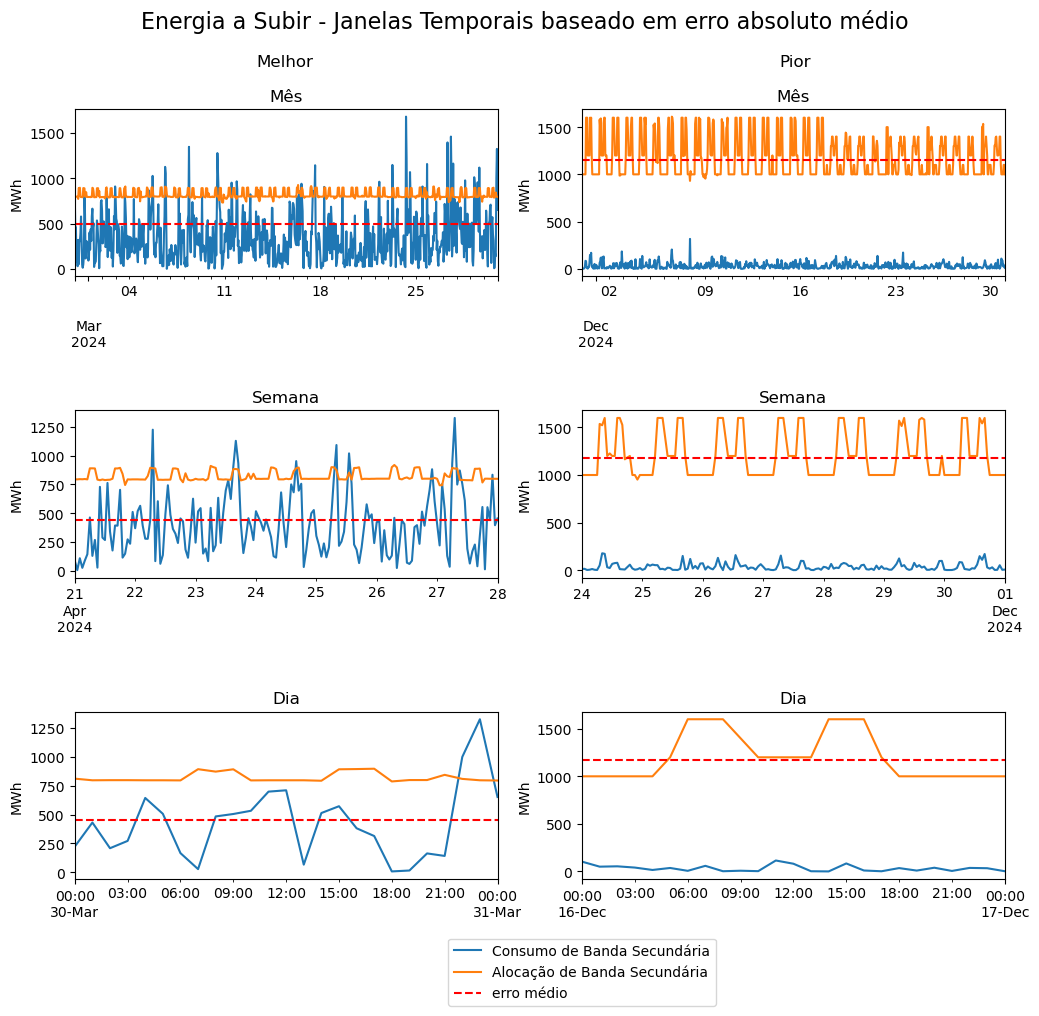
\includegraphics[width=\textwidth]{plots/alocacoes_temporais_upward_dataset.png}
    \caption{Janelas temporais de benchmark energia a subir}
    \label{fig:benchmarktimewindowsup}
\end{figure}


\begin{figure}[H]
    \centering
    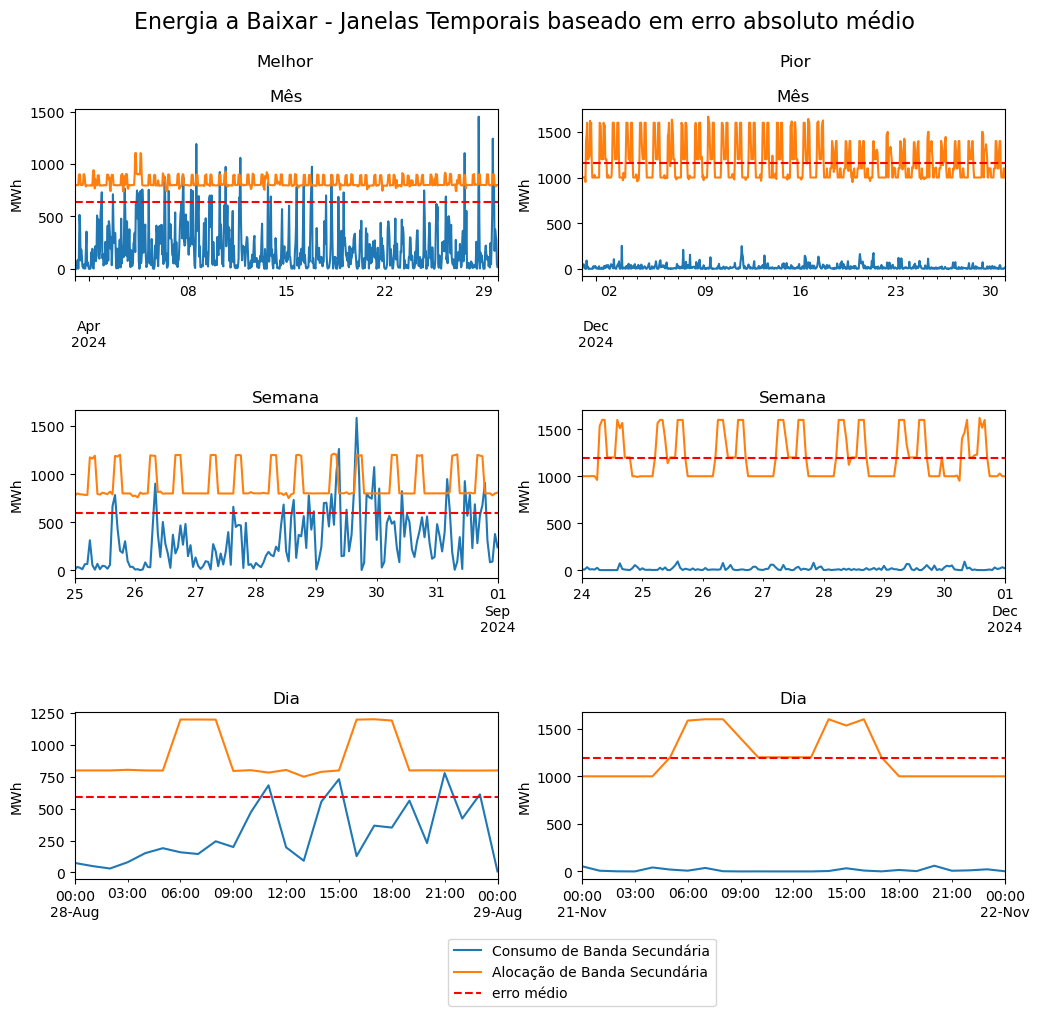
\includegraphics[width=\textwidth]{plots/alocacoes_temporais_downward_dataset.png}
    \caption{Janelas temporais de benchmark energia a descer}
    \label{fig:benchmarktimewindowsdown}
\end{figure}

Dentro destas janelas temporais conseguimos ter melhor a percepção da natureza estática deste modelo actual, e qual longe está dos valores reais necessários.\\


